\documentclass[12pt,a4paper]{article}
\usepackage{amsmath}
\usepackage[english]{babel}
\usepackage{graphicx}
\usepackage{listings}
\usepackage{fullpage}
\usepackage[T1]{fontenc}
\usepackage{enumerate}
\usepackage[makeroom]{cancel}
\usepackage{hyperref}
\usepackage{natbib}
\bibliographystyle{apj}

\lstdefinestyle{custompython}{
  belowcaptionskip=1\baselineskip,
  breaklines=true,
  frame=L,
  xleftmargin=\parindent,
  language=bash,
  basicstyle=\footnotesize\ttfamily,
  showstringspaces=false,
  %commentstyle=\itshape\color{purple!40!black},
  %keywordstyle=\itshape\color{green!40!black},
  %identifierstyle=\color{blue},
  %stringstyle=\color{orange},
}

\usepackage{todonotes}
\newcommand\TM[1]{\todo[color=green!40, inline, size=\small]{TM: #1}}
\newcommand\EW[1]{\todo[color=blue!40, inline, size=\small]{TM: #1}}
\newcommand\LC[1]{\todo[color=magenta!40, inline, size=\small]{TM: #1}}

% Roman numerals command
\makeatletter
\newcommand*{\rom}[1]{\expandafter\@slowromancap\romannumeral #1@}
\makeatother

% Some definitions for writing SN, SNe, SN Ia, and SNe Ia...
\newcommand{\sn}{\mbox{SN}}
\newcommand{\sne}{\mbox{SNe}}
\newcommand{\sna}{\mbox{SN \rom{1}a}}
\newcommand{\snea}{\mbox{SNe \rom{1}a}}

\author{
  Cheng, Lidens\\
  \texttt{lidenscheng@email.arizona.edu}
  \and
  McClintock, Tom\\
  \texttt{tmcclintock@email.arizona.edu}
  \and
  Wagoner, Erika\\
  \texttt{wagoner47@email.arizona.edu}
}
\title{Astr 513: Final Project}

\begin{document}
\maketitle

\section{Type Ia Supernovae}
\TM{TODO: Complete this section.}

\section{Data}
\label{sec:data}
\TM{TODO: Complete this section.}
Our data is compiled from \citet{betoule2014} and \citet{rest2014} blah blah blah...

\subsection{The JLA sample}
\label{sec:betoule}

\citet{betoule2014} define their ``joint light-curve analysis'' (JLA) 
sample, a total of 740 type Ia supernovae (SNe Ia) 
%If we define the abbreviations elsewhere, this can change -- ELW
compiled from a combination of data from the Sloan Digital Sky 
Survey (SDSS), the Supernova Legacy Survey (SNLS), the Hubble Space 
Telescope (HST), and several other experiments. The 613 SDSS \snea{} 
come from the SDSS supernova survey (SDSS-SNS) of SDSS-II \citep{sako2014} 
with redshifts of $0.05 < z < 0.4$, and 374 of them are selected from those 
that were confirmed in the spectroscopic follow-up. The rest of the 
\sne{} come from the compilation by \citet{conley2011}, which includes 
242 spectroscopically confirmed \snea{} from SNLS at redshifts $0.2 < z < 1$, 
14 \snea{} from HST at very high redshifts of $0.7 < z < 1.4$, and 123 
low redshift ($z < 0.08$) from a variety of sources. We made use of the 
publicly available distance moduli, redshifts, and covariance 
matrix provided by \citet{betoule2014}\footnote{Data is available 
for download via \url{http://cdsweb.u-strasbrg.fr/cgi-bin/qcat?J/A+A/568/A22}}. 
We note that the distance moduli are binned, so that they are only computed and 
given on a grid of redshifts. The distance modulus can then be well 
approximated by a piecewise linear function of $\log(z)$ that is given 
in a single redshift bin $z_b \le z < z_{b+1}$ as 
\citep[see][Appendix E.1]{betoule2014}
\begin{equation}
\label{eq:binnedMu}
\bar{\mu}(z) = (1 - \alpha) \mu_b + \alpha \mu_{b+1},
\end{equation}
where they have defined 
$\alpha = \log\left(\frac{z}{z_b}\right)/\log\left(\frac{z_{b+1}}{z_b}\right)$ 
and $\mu_i$ is the distance modulus at control point $z_i$. 
Therefore, the data and covariance matrix are merely given at the 
31 control points log-spaced in the redshift range $0.01 < z < 1.3$.

\subsection{Covariances}
\label{sec:covariances}
\TM{A subsection that explains how the covariance matrix looks. Basically
  a brief discussion about how it was made and then a picture of the 
  {\it correlation} matrix. Example figure below.}

\begin{figure}
 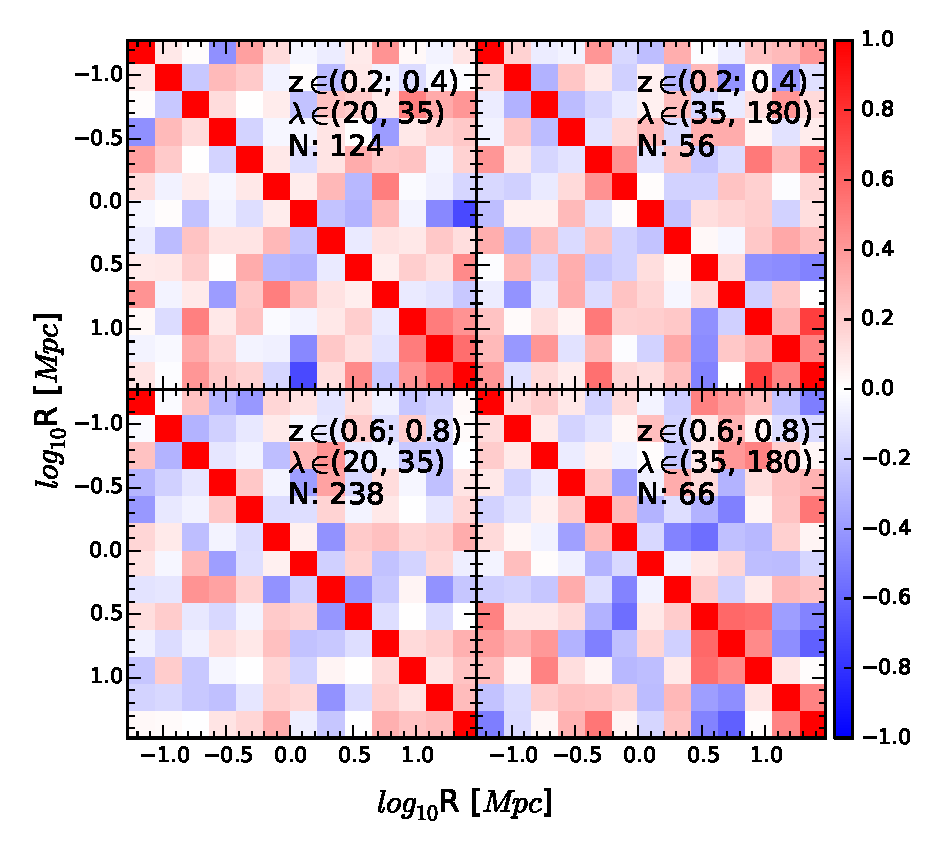
\includegraphics[width=\linewidth]{figures/clusters-randoms_noqc_correlation_subset.eps}
 \caption{Correlation matrix example. We will just have one panel.}
 \label{fig:cmatrix}
\end{figure}

\section{$\mu$ Model}
\label{sec:model}
\TM{This explains how to go from a cosmology to $\mu(z)$.}

\subsection{Likelihood}
\label{sec:likelihood}
\TM{This has our likelihood.}

%\section*{References}
%
%\begin{enumerate}
%  \item test
%\end{enumerate}

\bibliography{final}

\end{document}
